\chapter{Dữ liệu về điện tim}
\thispagestyle{fancy}

\section{MIT-BIH Arrhythmia Database}
\subsection{Giới thiệu}
Bộ dữ liệu Loạn nhịp tim MIT-BIH là một trong những bộ dữ liệu về điện tim nổi tiếng nhất, được sử dụng phổ biến ở rất nhiều các nghiên cứu về điện tim trên toàn thế giới. Bộ dữ liệu được thu thập từ những trung tâm y tế, nghiên cứu hàng đầu qua nhiều công đoạn xử lý tín hiệu và được xem xét bởi những y bác sĩ uy tín. Bộ dữ liệu thể hiện rõ những bất thường tim mạch cũng như có những ghi chú chi tiết trên từng bệnh nhân đem lại cho nhưng nghiên cứu khoa học một nguồn tư liệu dồi dào và chính xác.
\subsection{Nguồn thu thập dữ liệu}
Physionet à một trang web truy cập miễn phí các bộ dữ liệu lớn về tín hiệu sinh lý được ghi lại (PhysioBank) và những phần mềm mã nguồn mở liên quan (PhysioToolkit).
\begin{center}
    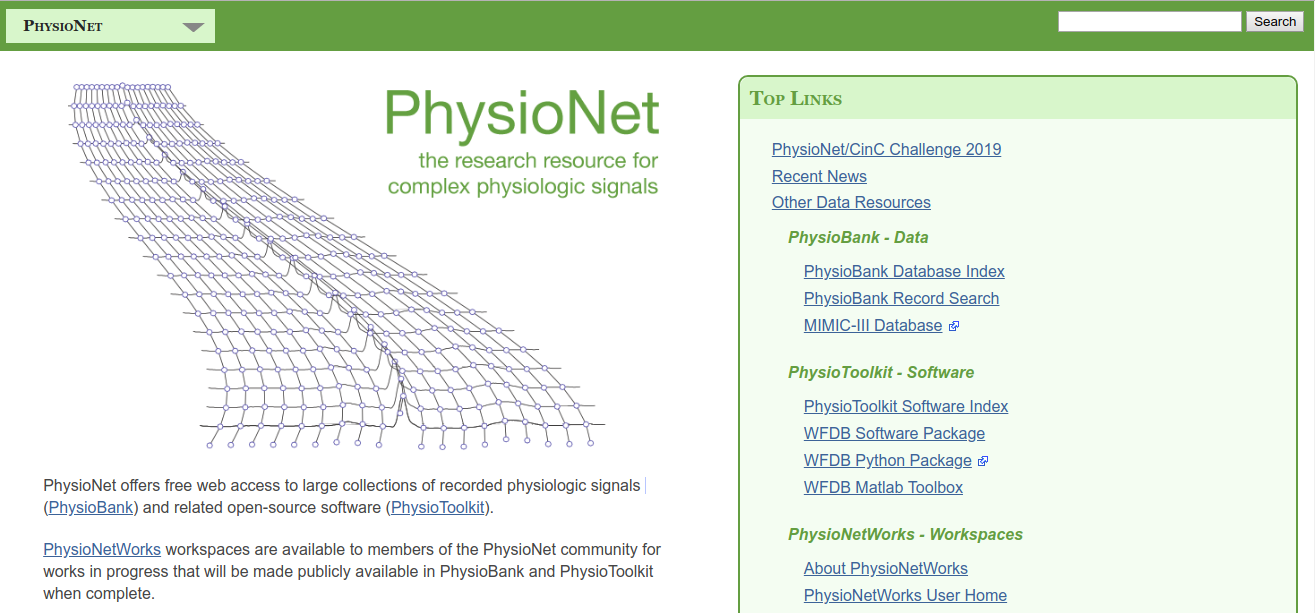
\includegraphics[scale=.3]{image/chapter2/Screenshot_from_2019-03-11_04-58-18.png}
    \begin{figure}[htp]
    \begin{center}
    \end{center}
    \caption{Trang Physionet}
    \end{figure}
\end{center}

\subsection{Thông tin về database}
Từ năm 1975, các phòng thí nghiệm tại Bệnh viện Beth Israel của Boston (nay là Trung tâm Y tế Beth Israel Deaconess) và tại MIT đã hỗ trợ nghiên cứu về phân tích rối loạn nhịp tim và các đối tượng liên quan. Một trong những sản phẩm chính đầu tiên của nỗ lực đó là Cơ sở dữ liệu Chứng loạn nhịp tim MIT-BIH, chúng tôi đã hoàn thành và bắt đầu phân phối vào năm 1980.\cite{mitbih}\par
Cơ sở dữ liệu Chứng loạn nhịp tim MIT-BIH chứa 48 trích đoạn nửa tiếng của các bản ghi ECG lưu động hai kênh, thu được từ 47 đối tượng được nghiên cứu bởi Phòng thí nghiệm Chứng loạn nhịp tim BIH từ năm 1975 đến 1979. Đối tượng là 25 nam từ 32 đến 89 tuổi và 22 nữ từ 23 đến 89 tuổi. Hai mươi ba bản ghi được chọn ngẫu nhiên từ bộ 4000 dữ liệu 24 tiếng Các bản ghi ECG lưu động  được thu thập từ một nhóm bệnh nhân nội trú hỗn hợp (khoảng 60\%) và bệnh nhân ngoại trú (khoảng 40\%) tại Bệnh viện Beth Israel của Boston; 25 bản ghi còn lại được chọn từ cùng một bộ để bao gồm các rối loạn nhịp tim ít phổ biến hơn nhưng có ý nghĩa lâm sàng sẽ không được thể hiện tốt trong một mẫu ngẫu nhiên nhỏ.\par
Nhóm đầu tiên được dự định là một mẫu đại diện cho sự đa dạng của dạng sóng và nhiễu mà một máy phát hiện rối loạn nhịp tim có thể gặp phải trong sử dụng lâm sàng thông thường. Các hồ sơ trong nhóm thứ hai đã được chọn để bao gồm rối loạn nhịp thất, rối loạn chức năng và thất trái phức tạp và bất thường dẫn truyền. Một vài trong số các hồ sơ này đã được chọn vì các đặc điểm của nhịp điệu, biến thể hình thái QRS hoặc chất lượng tín hiệu có thể được dự kiến sẽ gây khó khăn đáng kể cho các máy phát hiện rối loạn nhịp tim; những hồ sơ này đã đạt được sự nổi tiếng đáng kể trong số những người sử dụng cơ sở dữ liệu.\par
Các bản ghi được số hóa ở 360 mẫu mỗi giây trên mỗi kênh với độ phân giải 11-bit trên phạm vi 10 mV. Hai hoặc nhiều bác sĩ tim mạch chú thích độc lập mỗi hồ sơ; những bất đồng đã được giải quyết để có được các chú thích tham chiếu có thể đọc được trên máy tính cho mỗi nhịp (khoảng 110.000 chú thích trong tất cả) kèm theo cơ sở dữ liệu.
% \begin{center}
%     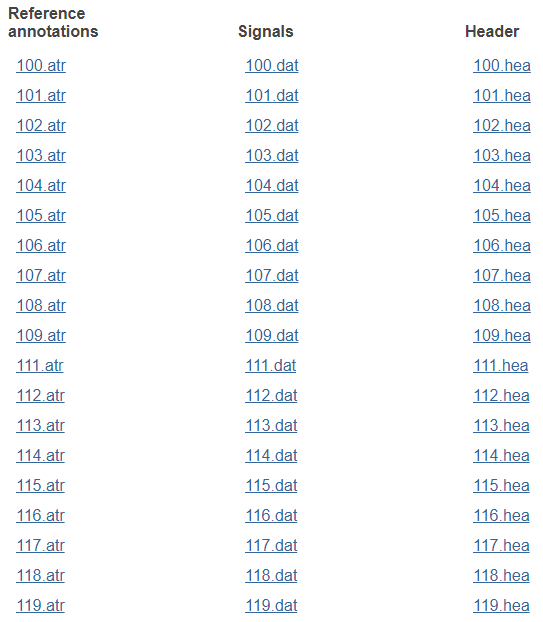
\includegraphics[scale=.4]{image/week3/mit.png}
%     \begin{figure}[htp]
%     \begin{center}
%     \end{center}
%     \caption{Dataset sample}
%     \end{figure}
% \end{center}
\subsubsection{Cấu trúc chuyển đạo và ghi chú}
\begin{center}
    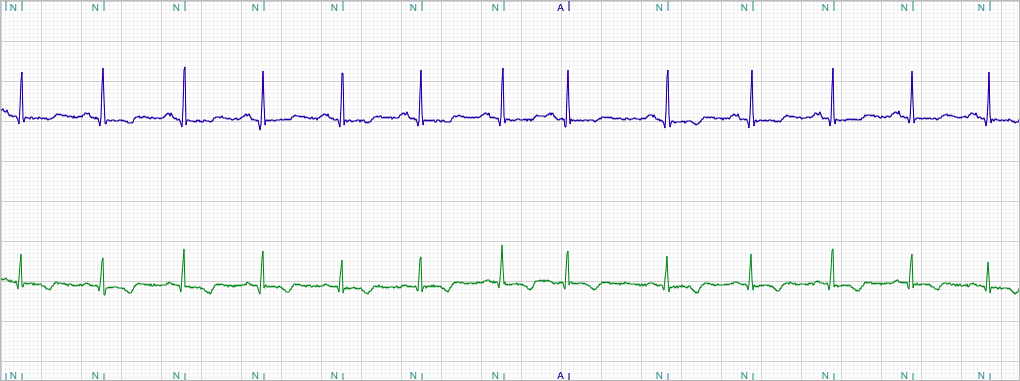
\includegraphics[scale=.4]{image/chapter2/100bee.png}
    \begin{figure}[htp]
    \begin{center}
    \end{center}
    \caption{Ghi chú trên bản ghi thứ 100}
    \end{figure}
\end{center}
Trong hầu hết các bản ghi, tín hiệu trên là modified limb lead II (MLII), thu được bằng cách đặt các điện cực trên ngực. Tín hiệu thấp hơn thường là đạo trình sửa đổi V1 (đôi khi V2 hoặc V5 và trong một trường hợp V4); đối với tín hiệu trên, các điện cực cũng được đặt trên ngực. Cấu hình này được sử dụng thường xuyên bởi Phòng thí nghiệm loạn nhịp tim BIH. Các phức bộ QRS bình thường thường nổi bật trong tín hiệu trên. Tuy nhiên, trục dẫn cho tín hiệu thấp hơn có thể gần trực giao với trục điện tim trung bình, tuy nhiên (tức là, nhịp đập bình thường thường là hai pha và có thể gần như đẳng điện). Do đó, nhịp đập bình thường thường khó phân biệt ở tín hiệu thấp hơn, mặc dù nhịp đập ngoài tử cung thường sẽ nổi bật hơn (xem, ví dụ, ghi 106). Một ngoại lệ đáng chú ý là bản ghi 114, trong đó các tín hiệu bị đảo ngược. Vì điều này thỉnh thoảng xảy ra trong thực hành lâm sàng, máy dò loạn nhịp tim nên được trang bị để đối phó với tình huống này. Trong hồ sơ 102 và 104, không thể sử dụng chì II đã được sửa đổi vì băng phẫu thuật trên bệnh nhân; chì V5 được sửa đổi đã được sử dụng cho tín hiệu trên trong các bản ghi này.\par
Tại mỗi đỉnh sóng R sẽ được đánh ghi chú cho sóng đó. Ban đầu bộ nhãn đánh dấu trên tập dữ liệu được tạo ra bằng một máy dò phức bộ QRS và đánh dấu nhịp đó là bình thường. Sau đó bộ dữ liệu được đánh nhãn lại. Mỗi bản ghi được đánh nhãn lại một cách chính xác hơn bằng những bác sĩ chuyên khoa tim mạch. Các bác sĩ đã thêm vào các nhãn bổ sung một cách chính xác hơn những nhãn đã đánh, các nhịp bị lỗi cũng như xóa các phát hiện sai lầm.

\subsubsection{Ghi chú trên tập dữ liệu}
\begin{center}
    \begin{tabular}{|c|c|}
         \hline
         Symbol & Meaning \\
         \hline
         . or N & Normal beat \\
         \hline
         L & Left bundle branch block beat \\
         \hline
         R & Right bundle branch block beat \\
         \hline
         A & Atrial premature beat \\
         \hline
         a & Aberrated atrial premature beat \\
         \hline
         J & Nodal (junctional) premature beat\\
         S & Supraventricular premature beat\\
         \hline
         V & Premature ventricular contraction\\
         \hline
         F & Fusion of ventricular and normal beat\\
         \hline
         [ & Start of ventricular flutter/fibrillation\\
         \hline
         ! & Ventricular flutter wave\\
         \hline
         ] & End of ventricular flutter/fibrillation\\
         \hline
         e & Atrial escape beat\\
         \hline
         j & Nodal (junctional) escape beat\\
         \hline
         E & Ventricular escape beat\\
         \hline
         / & Paced beat\\
         \hline
         f & Fusion of paced and normal beat\\
         \hline
         x & Non-conducted P-wave (blocked APB)\\
         \hline
         Q & Unclassifiable beat\\
         \hline
         | & Isolated QRS-like artifact\\
         \hline
    \end{tabular}
\end{center}

\subsubsection{Thông tin trên từng bệnh nhân}
Mỗi bệnh nhân (bản ghi) được lưu lại từng thông tin về: Độ tuổi, giới tính, thuốc sử dụng trong quá trình điều trị, thống kê về nhịp, những ghi chú đối với những đoạn ECG quan trọng trong nghiên cứu,...
\begin{center}
    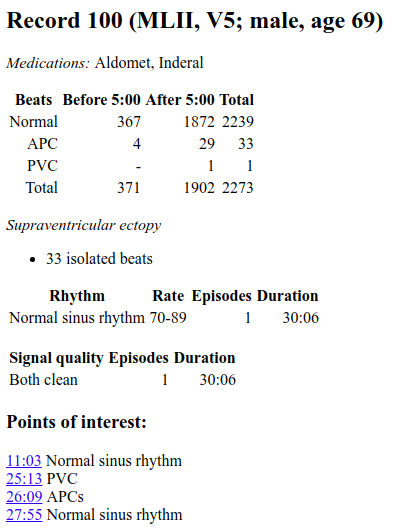
\includegraphics[scale=.4]{image/chapter2/record_info.png}
    \begin{figure}[htp]
    \begin{center}
    \end{center}
    \caption{Thông tin bệnh nhân (bản ghi thứ 100)}
    \end{figure}
\end{center}